\section{Konzept}


\subsection{Überblick}
Ludwig Systems benötigt eine Lösung, welche von der Traverse aus die Ist-Koordinaten, die Rotation und Neigung der Last ausgibt. Das Konzept soll dieses Ziel erfüllen um in der Zukunft die Traverse automatisch bewegen zu können. Des Weiteren soll das Konzept sicherstellen, dass die Genauigkeiten ,welche vom Kunden gegeben wurde, eingehalten werden können. 
Da sich die Art von Last ändern kann, wurde der Fokus auf die Lokalisierung der Anschlagspunkte gelegt. 
Es wurden 2 Konzepte ausgearbeitet, welche diese Ziele erfüllen können. Beim ersten Konzept wird ein Machine-Learning Modell benutzt um die Anschlagspunkte zu erkennen und 3D Lokalisierung durchzuführen und beim zweiten Konzept werden die Anschlagspunkte durch AR Marker 
Lokalisiert.


\subsection{Konzept: Lokalisierung durch Machine Learning}

In diesem Konzept geht es darum die Anchlagspunkte mithilfe von Objekterkennung durch YOLO zu erkennen und die Ist-Koordinaten durch 3D Lokalisierung zu erhalten. 
Für dieses Konzept wird ein Machine Learning Modell benötigt, welches diese Aufgabe erfüllen kann. 
Weiters würden gelabelte Bilder von den Lasten und Anschlagspunkte zum Lernen und weitere Bilder zum Testen benötigt.

\subsection{Konzept: Lokalisierung durch AR Marker}

In diesem Konzept geht es darum die Anschlagspunkte durch AR Marker, wie ArUco oder AprilTags, zu lokalisieren. Dabei werden die Marker um den Anschlagspunkt angeordnet. Wenn die Marker dann erkannt werden, kann durch Posenschätzung die 3D Koordinaten und 3D Rotationen berechnet werden. Durch die Anordnung der Marker kann dann die 3D Koordinaten vom Anschlagspunkt berechnet werden. 
Für dieses Konzept werden Sticker von den Markern benötigt, welche eine genaue Grösse haben. 

\subsubsection{Marker Anordnung}

Wie in der Abbildung (ref) zu sehen ist werden 4 Marker in einem Kreuz-Muster um den Anschlagspunkt angeordnet. Für Anschlagspunkt 1 werden Marker mit den IDs von 0 bis 3 benutzt und in der Reihenfolge links, oben, rechts und dann unten angeordnet. Für Anschlagspunkt 2 Marker mit den IDs von 4 bis 7 benutzt. Dadurch können zwischen den zwei Anschlagspunkten differenziert werden wenn beide Anschlagspunkte im Bild sind.Falls weitere Anschlagspunkte benötigt werden, sollten die Marker-IDs-Reihenfolge und Position fortgeführt werden. Diese Anordnung sorgt dafür dass mindestens ein Marker erkannt werden kann, soweit die Traverse in der definierten Grenze ist. 
(redundanz erhöht stabilität)

\clearpage
\subsubsection{Markergröße}

Die Markergröße ist von entscheidender Bedeutung, um die Anschlagspunkte präzise 
zu lokalisieren und die Berechnungen für die Ausrichtung der Traverse durchzuführen. 
Ziel ist es, den Marker so groß wie möglich zu gestalten, um die Genauigkeit der 
Distanzberechnung zu maximieren. Abbildung \ref{fig:marker} veranschaulicht, wie die Markergröße 
basierend auf einem gegebenen Radius \( R \) maximiert werden kann.

\begin{figure}[H]
    \centering
    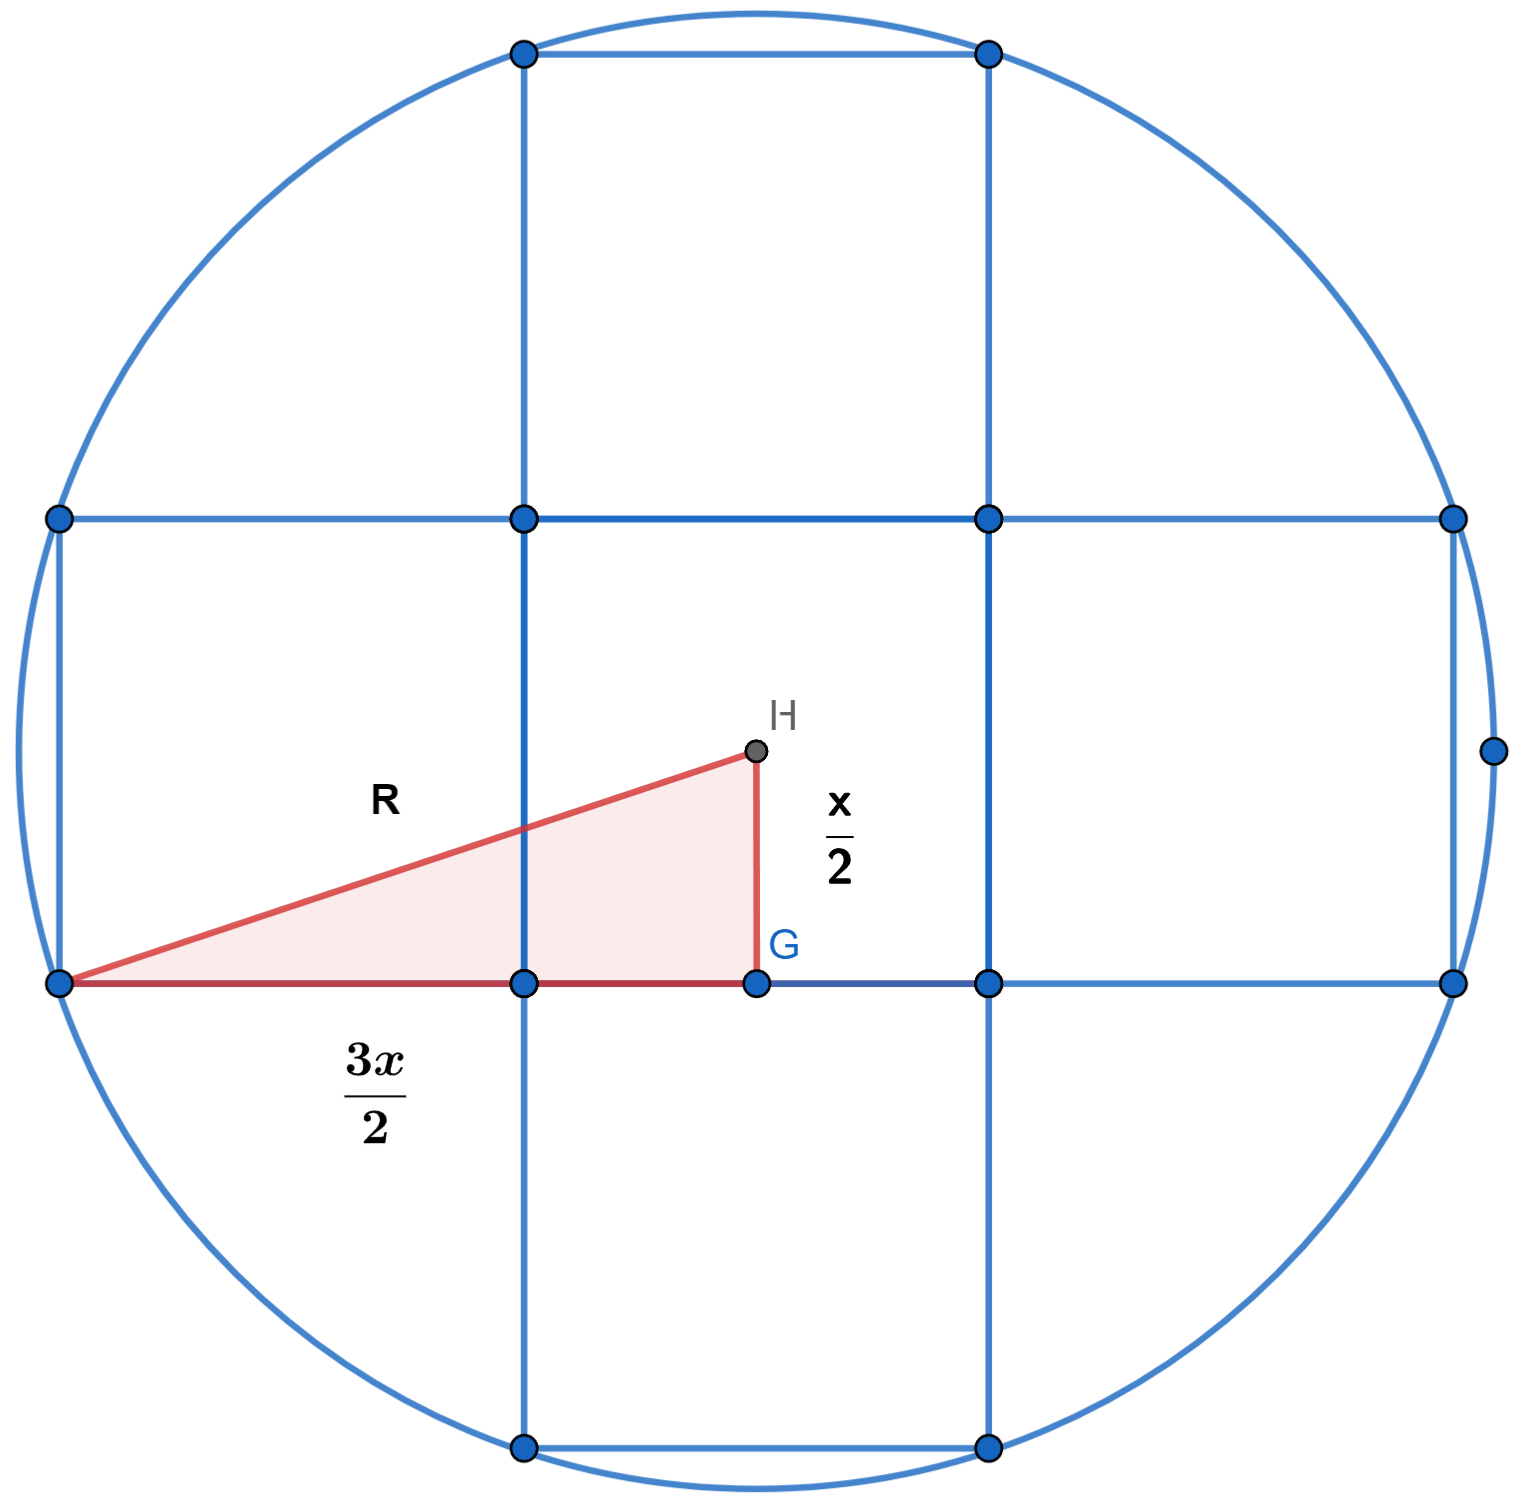
\includegraphics[width=\linewidth]{graphics/marker.png}
    \caption{Diagramm zur Berechnung der Markergröße}
    \label{fig:marker}
\end{figure}

Um die Fläche der Marker (dargestellt als blaue Quadrate) zu maximieren, berechnen wir die Fläche des Quadrats unter Berücksichtigung der Teilflächen. Die Gesamtfläche des Kreises wird durch die folgende Formel beschrieben:

\[
A_\text{Kreis} = \pi \cdot R^2
\]

Die Fläche eines einzelnen Quadrats ergibt sich aus:

\[
A_{\text{Quad}} = x^2
\]

Die Fläche der vier kleinen und vier großen Kreissegmente wird mithilfe der folgenden Formel berechnet:

\[
A_\text{Kreisegment} = \frac{1}{2} \cdot R^2 \cdot (\alpha - \sin(\alpha))
\]

Dabei kann der Winkel \(\alpha\) über die Sehnenlänge \(c\) berechnet werden, die in Abbildung \ref{fig:marker} in Rot und Schwarz dargestellt ist. Üblicherweise wird \(c\) in der Literatur als Sehnenlänge bezeichnet:

\[
c_\text{klein} = x
\]

\[
c_\text{gross} = \sqrt{2} \cdot x
\]

Der Winkel \(\alpha\) ergibt sich aus der folgenden Beziehung:

\[
\alpha = 2 \cdot \arcsin\left(\frac{c}{2R}\right)
\]

Mithilfe der berechneten Teilflächen kann nun eine quadratische Funktion konstruiert werden, die die Beziehung zwischen der Markergröße und dem gegebenen Radius \(R\) beschreibt. Um die maximale Fläche zu ermitteln, lösen wir die Gleichung durch Bestimmung der Nullstellen:

\[
f(x) = 7 \cdot A_\text{Quad} + 4 \cdot A_\text{SegKlein} + 4 \cdot A_\text{SegGross} - \pi \cdot R^2
\]


\subsubsection{Mittelpunkt-Berechnung der Marker Anordnung}

Um von den 3D Koordinaten der Markern zu den 3D Koordinaten vom Anschlagspunkt zu kommen, muss eine Translation gemacht werden. Da die Berechnung zum Mittelpunkt auch mit nur einem Marker funktionieren muss, wird von jede Marker-Koordinaten in die Mitte des Keuz-Musters translatiert. Die Anordung der Marker und die damit zusammenhängende Marker-ID bestimmt welche Translation durchgeführt werden muss. Marker mit der ID 0 und 4 werden um + l und Marker mit ID 2 und 6 um -l in der X-Achse translatiert. Marker mit der ID 1 und 5 werden um -l und Marker mit ID 3 und 7 um +l in der Y-Achse translatiert. Falls mehrere Marker erkannt werden, wird der Mittelwert aller neuen Punkten genommen.

\subsection{Evaluation Konzepte}
Um die Lokalisierung durch Machine-Learning durchzuführen braucht es genügend gelabelte Bilder um ein Modell zu trainieren, da kein vortrainiertes Modell vorhanden ist. Das auftreiben und labeln von diesen Bildern würde Zeit und Kosten brauchen. Des Weiteren kann nicht sicher gestellt werden, dass die 3D Koordinaten und Rotationen denn gewünschten Genauigkeiten entsprechen. Die Kunden bestätigten das Marker an der Last angebracht werden können und dass sichergestellt werden kann dass diese den gleichen Abstand zueinander haben, weshalb das zweite Konzept ausgewählt wurde.


\subsection{System Anforderungen}

\subsubsection{Lokalisierung Last}
(Erklärung wie die Lokalisierung mithilfe von Marker funktionieren sollte.)


\subsubsection{Distanzberechnung}
\subsubsection{Kameraposition}

\subsection{Kamera Anforderungen}
\subsubsection{Kamera Spezifikationen}
(Erklärung welche Kamera Eigenschaften gebraucht werden und wieso wir diese brauchen.)

\subsubsection{Kamera Eigenschaften}
(Erklärung der Rechnung horizontale Bildauflösung und auflistung aller Eigenschaften ausgehend von der Mindest distanz.)



